\documentclass[12pt]{article}

\usepackage{fullpage}
\usepackage{graphicx, rotating, booktabs} 
\usepackage{times} 
\usepackage{natbib} 
\usepackage{indentfirst} 
\usepackage{setspace}
\usepackage{grffile} 
\usepackage{hyperref}
\usepackage{adjustbox}
\usepackage{amsmath}
\usepackage{siunitx}
\usepackage{multirow}
\setcitestyle{aysep{}}


\singlespace
\title{\textbf{Democracy and Alliance Treaty Depth}}
\author{Joshua Alley\footnote{Graduate Student,
Department of Political Science, Texas A\&M University.}}
\date{\today}

\bibliographystyle{apsr}

\begin{document}

\maketitle 

\doublespace 

\begin{abstract}
Why do states form deep alliances? 
I argue that alliances between democracies tend to have greater treaty depth as members add defense coordination and cooperation to promises of military support. 
Democratic states use treaty depth to reassure allies, because depth has fewer domestic audience costs than unconditional military support, but it is still a costly signal of reliability.
To test this claim, I implement a series of statistical models and offer a short case study of the North Atlantic Treaty Organization.
I find that as the average polity score of alliance members at the time of formation increases, treaty depth increases, but there is mixed evidence that allied democracy decreases the probability the treaty offers unconditional military support. 
Thus, democracies offer moderate commitments with some treaty depth and perhaps some conditions on military support. 
The argument and findings challenge claims that democracies prefer limited alliance commitments. 
\end{abstract}


\newpage 


\section{Introduction}


% Start with hook: maybe a story of a deep and shallow alliance 
Why do states make deep alliance treaties? 
While some alliance treaties only include a promise of military support, others supplement military support with commitments of extensive defense cooperation. 
To give a well-known example, the NATO treaty commits to setting up a formal international organization to govern the alliance. 


Treaty depth is a common policy choice with important consequences. 
At least half of all ATOP alliances with offensive or defense obligations have some treaty depth.
Deep alliances encourage non-major power members to reduce military spending because treaty depth adds credibility.  
On the other hand, participation in shallow alliances increases non-major power military spending because states use military spending to hedge against abandonment.
Thus, treaty depth affects alliance politics by shaping treaty credibility and the distribution of military spending burdens among members. 


% Describe question and contribution of the paper
Despite the consequences of alliance treaty depth, we have little idea when states add depth to their alliances.\footnote{\citet{Mattes2012} examines the causes of military institutionalization.}
In this paper, I explain when states make deep alliance treaties.
I argue that domestic politics shape how states use unconditional military support and treaty depth to establish credible alliance commitments. 
Alliance negotiations center on whether prospective members will offer military support and conditions on that support \citep{Poast2019a}. 
When alliance members are unwilling to offer unconditional military support, depth provides an alternative source of reliability.
Democracies prefer to reassure allies with treaty depth because unconditional military support exposes them to the audience costs of treaty violation and limited commitments are harder to violate \citep{Mattes2012, Chibaetal2015}.
At the same time, these limited alliances can increase allied fears of abandonment. 
Therefore, democracies use the costly provisions in deep alliances to reassure their partners because treaty depth is less salient in domestic politics than military interventions. 
Democratic regimes' use of treaty depth is analogous to their ``optimal obfuscation'' in trade policy \citep{Kono2006}. 


Because depth and unconditional promises of military support both increase treaty credibility, I examine how these aspects of alliance treaty design are related. 
I combine depth and unconditional military support to classify alliances as weak, strong, or moderate commitments. 
Alliances with both depth and unconditional support are particularly strong commitments on paper--- they include high peacetime costs and higher odds that the treaty will be invoked. 
Weak alliance commitments lack depth and only provide conditional military support. 
Moderate strength commitments have depth or unconditional military support. 
My argument suggests that democracies prefer moderately strong alliances with depth and conditional military support.  


I test the argument with several statistical models and an illustrative case study of the North Atlantic Treaty Organization (NATO).
The statistical models connect decisions about treaty depth and unconditional military support and adjust for unobservable correlates of the two processes \citep{Braumoelleretal2018}. 
The case study checks the theoretical process and statistical results \citep{SeawrightGerring2008, Seawright2016}. 
I find consistent evidence that greater allied democracy at the time of alliance formation increases treaty depth.
Evidence that democratic membership decreases the probability of unconditional military support is less consistent, however. 


% Para on implications: sources of credibility and reassurance are connected
The argument and findings have important consequences for research on alliance treaty design. 
Existing scholarship examines parts of treaty design in isolation \citep{Benson2012, Mattes2012, Chibaetal2015}, but different sources of credibility in alliance treaty design are connected. 
Theories and models that consider one alliance characteristic at a time may generate misleading conclusions. 
For example, previous estimates of the connection between democracy and treaty depth produced null findings, perhaps because they did not jointly model treaty depth and conditions on military support. 


% Paragraph on the importance of democracy in alliance pol
This paper also adds to knowledge of how domestic politics affect alliance politics. 
Scholars have long acknowledged that democracy and alliances are connected \citep{LaiReiter2000, GiblerWolford2006, Mattes2012, Warren2016, McManusYarhi-Milo2017}. 
Existing scholarship suggests that democracies prefer limited commitments \citep{Mattes2012, Chibaetal2015} because they are more likely to make conditional promises of military support. 
\citet{Chibaetal2015} write that ``domestic costs can make democratic states wary of engaging in agreements requiring broad and/or deep cooperation.'' 
My argument suggests that although democracies screen the scope of their commitments carefully, they form deeper alliances on other dimensions.  
Scholars often claim that audience costs make democratic commitments are more credible \citep{Gaubatz1996, Leedsetal2009, DigiuseppePoast2016}, but this relationship is disputed \citep{GartzkeGleditsch2004, DownesSechser2012}. 
The net effect of the connection between democracy, alliance design and treaty credibility requires further research. 


More generally, this paper contributes to a rich literature on domestic politics and international cooperation, e.g. \citep{DownesRocke1995, Fearon1998, Leeds1999, MattesRodriguez2014}. 
In particular, I show that democracies form deep security institutions because these are less salient for voters. 
Audience costs sometimes push democracies to obfuscate the limits of their international commitments. 


% roadmap for the paper 
The paper proceeds as follows. 
In the next section, I lay out the argument and hypothesis. 
Then I describe the data and research design. 
Following that, I provide empirical evidence from several statistical models and a case study of NATO. 
The final sections discuss the results and implications. 


\section{Argument}


In this argument, I start by defining treaty depth. 
Then, I offer a brief review of existing work on alliance treaty design to show that scholars have paid little attention to treaty depth.  
After that, I describe a general model of alliance treaty negotiations. 
Finally, I explain how alliance negotiations with democracies often increase treaty depth, but make unconditional military support less likely. 


% define alliance treaty depth
Alliance depth is the extent of defense cooperation formalized in the treaty. 
Deep alliances require additional military policy coordination and cooperation. 
While shallow alliances stipulate more arms-length ties between members, deep treaties lead to closer cooperation through intermediate commitments that fall between treaty formation and military intervention. 
Defense cooperation in a deep alliance takes many forms. 
Allies can form an integrated military command, provide military aid, commit to a common defense policy, provide basing rights, set up an international organization or undertake companion military agreements. 


% note that I'm the first one to address this question: lit review. 
Depth is therefore an important part of alliance treaty design.
Alliances are self-enforcing contracts or institutions \citep{Leedsetal2002, Morrow2000}.
Given external threats in an anarchic international system, states form alliances to aggregate military capability and secure their foreign policy interests \citep{Altfield1984, Smith1995, Snyder1997, FordhamPoast2014}. 


Potential alliance members can design a wide range of treaties \citep{Leedsetal2000, Leedsetal2002, Benson2012, BensonClinton2016}. 
Treaty design then shapes the costs and benefits of treaty participation. 
Beyond the benefit of potential military support, alliances also clarify international alignments \citep{Snyder1990} and support economic ties \citep{Gowa1995, Li2003, Long2003, Fordham2010, WolfordKim2017}. 
The costs of alliances include lost foreign policy autonomy \citep{Altfield1984, Morrow2000, Johnson2015}, and the potential consequences of opportunistic behavior. 
Opportunism in alliances includes abandonment, or the failure of alliance members to honor their commitments \citep{Leeds2003a, BerkemeierFuhrmann2018}, entrapment in unwanted conflicts \citep{Snyder1984}, and free-riding \citep{Morrow2000}.   


% Depth is understudied
States use treaty design to address abandonment and entrapment concerns. 
Despite its importance for alliance politics, the process of alliance treaty negotiation and design is understudied \citep{Poast2019a}. 
Scholars have paid more attention to conditions on military support, leaving little work on treaty depth. 


\citet{Mattes2012} examined alliance treaty design by using symmetry of capability and history of violation to explain conditions on military support, issue linkages, and military institutionalization in bilateral alliances. 
The measure of military institutionalization in this paper \citep{LeedsAnac2005} is close to my conceptualization of treaty depth, and Mattes finds that symmetric alliances where one partner have higher institutionalization. 
While checking the validity of their latent measure of treaty depth, \citet{BensonClinton2016} find that foreign policy agreement, major power involvement and treaty scope are all positively correlated with depth. 
Their latent measure of scope is based on the type of military support offered and conditions on that support. 
Benson and Clinton's latent measure of depth includes secrecy and issue linkages, so it is slightly different from my measure of defense cooperation. 
Following \citet{Mattes2012} and \citet{Poast2012}, I treat issue linkages as a separate from peacetime defense cooperation.


Unlike treaty depth, scholars have paid more attention to when states offer conditional military support. 
\citet{Benson2012} shows that foreign policy disagreements and revisionist protege states increase the likelihood of limited military support.
\citet{Mattes2012} finds that joint democracy increases the probability of conditional alliance obligations, as well as little evidence that alliance symmetry and history of violation affect conditionality. 
\citet{Chibaetal2015} added to to existing work on limited obligations by showing that democracies are more likely to form alliances with conditional military support or consultation. 


While research on depth and conditionality both deals with how states make credible alliance commitments, existing scholarship does not connect these different sources of reliability.  
\citet{Mattes2012} studies military institutionalization and conditionality as separate sources of reliability. 
Her argument and research design treat depth and institutionalization as independent.
Though \citet{BensonClinton2016} use scope to predict depth and depth to predict scope, they do not offer a joint model of these two facets of alliance treaty design. 
Perhaps as a result of these theoretical and empirical choices, both works find no association between the democracy of alliance members and treaty depth. 


Because states can use different foreign policy instruments as substitutes or complements to reach their goals \citep{Starr2000, MorganPalmer2000}, treaty depth and conditions on military support are probably related. 
My argument places depth and conditions on military support in a unified theoretical and empirical framework.\footnote{Other work by \citet{Poast2012, Poast2013} establishes that states often use issue linkages to facilitate alliance formation. Currently, I leave issue linkages aside in order to focus on how regime type shapes alliance treaty design. Leaving out issue linkages also simplifies the argument and research design.}
In the next section, I describe the general process of the argument, which connects domestic political regimes with treaty depth and conditionality. 


\subsection{Alliance Negotiations and Obligations}


% process of alliance negotiations: once agreed on military support, need to bolster. 
Alliance treaty design is the result of negotiations between members \citep{Poast2019a}, where states determine conditions on military support and treaty depth.
Both parts of treaty design address the benefits and costs of alliance participation, albeit in different ways.
Establishing if and when to offer military support is the essential task for potential alliance partners. 
Promises of military intervention are the core of alliances. 
To form an alliance, the members must have sufficient overlap in foreign policy interests \citep{Morrow1991, Smith1995, FordhamPoast2014}, especially their proposed war plans \citep{Poast2019a}.  


Promises of military support in an alliance vary widely, however. 
Shared foreign policy interests shape whether alliance members commit to unconditional or conditional military support.
Conditional alliances limit promises of intervention to particular regions, conflicts, or instances of non-provocation \citep{Leedsetal2000}, which reflects less overlap in foreign policy interests. 
When alliance members fear entrapment in unwanted conflicts, they constrain military support to specific circumstances \citep{Kim2011, Benson2012}.\footnote{Such deliberate design of alliances means clear instances of entrapment are rare \citep{Kim2011, Beckley2015}.} 
Conversely, offering unconditional military support is a strong signal of shared foreign policy interests. 
Attaching no conditions to a promised intervention means alliance members hazard the reputational \citep{Gibler2008, Crescenzietal2012} and audience \citep{Fearon1997} costs of treaty violation from many potential conflicts. 
Accepting these potential costs implies that fighting with allies in many circumstances is acceptable.
As such there is less fear of entrapment and many shared foreign policy interests. 
Therefore unconditional alliances are a key source of credibility, because they are a costly signal of substantial foreign policy agreement. 


% Part 2: depth
Alliance partners also negotiate over how to reinforce promises of military support and put them into action. 
This determines the depth of the treaty and provides additional evidence of alliance reliability. 
Depth shapes the perceived reliability of an alliance by providing opportunities for states to fulfill treaty obligations in peacetime \citep{Morrow1994}. 
When states implement deep obligations, it provides a costly signal of credible commitment. 
Implementing deep treaty provisions can also enhance joint war-fighting. 


% clarify difference in costs
Though depth and unconditional military support both increase alliance credibility, they have different costs. 
Conditions on military support do not change without a treaty renegotiation, and the costs of fighting is hypothetical unless the alliance is invoked.  
Alliance members and other states use the potential costs of military support to assess treaty reliability. 
Highly conditional alliances are less costly in expectation, which reduces their credibility. 
Conversely, the costs of depth can be observed without invoking promises of military support. 
Depth addresses time-inconsistency problems from changing foreign policy interests, which are a major threat to alliance fulfillment \citep{LeedsSavun2007}. 
Under a deep alliance treaty, members can use implementation of defense cooperation and policy coordination to assess allied reliability. 
Observing that alliance members adhere to peacetime promises indicates they will also honor promises of military support. 


% Combine the two: strong/weak/moderate
Treaty depth and unconditional military support are related because they both generate credibility. 
States could use depth as a substitute source of reliability, or to complement promises of unconditional military support. 
Prospective alliance members could also design an arms-length alliance commitment with neither depth nor unconditional military support. 
\autoref{tab:str-table} summarizes the possible combinations of depth and unconditional military support in alliance treaties. 
Strong alliances combine depth and unconditional military support, while weak alliances have neither. 
Moderate alliance commitments have one source of credibility. 


\begin{table}[hbt!]
\begin{center}
\caption{Potential alliance treaty strength based on treaty depth and conditions on military support.}
\begin{tabular}{ccc} 
                 & Conditional & Unconditional \\
\toprule
          Deep   &  Moderate & Strong \\
         Shallow & Weak      & Moderate \\
 \bottomrule
\end{tabular}
\label{tab:str-table}
\end{center} 
\end{table}


If strength combines depth and unconditional military support, why not analyze strength directly? 
I separate depth and unconditional military support for two reasons. 
First, they provide credibility in different ways, so states can decide to form alliances with one, both, or neither of depth and unconditional support.  
Second, existing research separates conditions on military support and depth. 


This connection between depth and conditions on military support means that understanding how domestic political regimes affect alliance treaty design must account for both sources of credibility.  
To start I accept the conventional wisdom that democracies are more likely to design alliances with conditional military support. 
As a result, democracies must then use greater treaty depth to address reliability concerns from these limited commitments.
I expect that as allied democracy rises, alliances will be more likely to have limited military support and high depth, leading to moderate overall commitment strength in alliances with more democratic membership. 


\subsection{Democratic Alliance Membership and Treaty Design}


% focus on average democracy 
How domestic political regimes affects alliance design depends on the prevalence of democratic states in alliance negotiations. 
To conceptualize the prevalence of democracies within an alliance, I focus on the average regime type of alliance members. 
As average democracy rises, the composition of the alliance becomes more democratic and members will have stronger preferences for using treaty depth to establish credible commitments.\footnote{I also follow \citet{Chibaetal2015} and conceptualize the weight of democracies in the alliance using the proportion of democracies. Using this measure leads to similar results- see the appendix for details.} 
More democratic membership will increase the likelihood of deep alliances with conditional obligations of military support. 


Democracies use treaty depth to reassure partners because it increases the perceived reliability of their alliances while shielding them from domestic audience costs. 
By including peacetime costs in a deep treaty, alliance members signal alliance reliability. 
Implementing costly promises of military aid, bases, or policy coordination indicates that alliance members are committed to the treaty. 
This increases allied confidence that democracies will honor their treaty obligations. 



Two characteristics of audience costs in democracies lead them to use treaty depth in alliance commitments.  
First, democratic leaders face high audience costs over promises of military support.
Democratic leaders fear that if they violate international commitments, public disapproval will lead to their removal from office. 
These audience costs increase as crises escalate \citep{Tomz2007}, so honoring promises of military support is highly salient. 
Second, the public in democracies lack sufficient information about foreign policy to monitor treaty depth. 
Treaty depth is a signal of commitment that allies can readily observe, but it has limited salience in domestic politics, which reduces audience costs. 
While military intervention is costly and highly public, peacetime alliance management is not.  
Democratic voters are unlikely to have much information or strong preferences about defense cooperation with allies. 
Although foreign policy elites may dispute changes in commitment to a deep alliance, such dissent is unlikely to translate into meaningful public opposition and electoral concerns.


% How do allies respond?
Unlike in domestic politics, differences in treaty depth and the implementation of alliance promises are salient in international politics. 
Allied states and potential adversaries pay careful attention to treaty depth. 
Therefore, democracies can use treaty depth to signal international commitment with less exposure to domestic audience costs. 


% analogous to optimal obfuscation in trade policy
The way democracies use treaty depth in alliances is analogous to their emphasis on non-tariff barriers in trade policy.
\citet{Kono2006} argues that because non-tariff barriers are more complex, voters lack sufficient information about their impact on consumer prices.
Tariffs, on the other hand, translate directly into prices in ways that are easy to understand.
The complexity of non-tariff barriers makes them less vulnerable to electoral attack, so democracies engage in ``optimal obfuscation'' and substitute non-tariff barriers for tariffs. 
In the same way, unconditional promises of military support and treaty depth both affect international relations, but the former is easily grasped by voters and the latter is not. 
Therefore, democratic leaders can use treaty depth to manage international relations, without as much exposure to domestic political blowback.


% What about different types of autocracies? 
The above argument uses the relative domestic audience costs of treaty depth and conditions on military support to explain why democracies often form deep alliances. 
How does this translate to autocracies? 
Some autocratic leaders, especially in single-party states, also face high audience costs for backing down in military conflicts due to scrutiny from domestic elites \citep{Weeks2014}. 
These domestic elites are highly informed, unlike the public in democracies, so they could impose costs on leaders that violate promises of treaty depth. 
In general, no type of autocracy has the exact mix of public information and high audience costs of military intervention as democracies, so leaving autocracies undifferentiated is sufficient for this paper. 
Examining heterogeneity among autocracies in alliance treaty design is a possible subject for future research. 


% express the key hypotheses
As a result of the lower audience costs of treaty depth, democracies will often design deep alliance treaties. 
As the average democracy of alliance members at the time of treaty formation increases, treaty depth should increase. 


\begin{quote}
\textsc{Treaty Depth Hypothesis: As the average democracy of alliance members at the time of formation increases, the depth of an alliance treaty will increase.}
\end{quote} 


% End with a well-established result: democracy and conditional obligations
I also expect that democractic alliance membership will reduce the probability of unconditional military support in the alliance treaty. 
The second claim is based on existing arguments and findings. 
\citet{Mattes2012} and \citet{Chibaetal2015} both show that democracies are more likely to design conditional alliances. 
They attribute this finding to higher audience costs of violating international commitments in democracies. 
Because democratic leaders face substantial audience costs from violating their international commitments, leaders design more limited commitments that are easier to fulfill. 
On the other hand, autocracies may be more willing to promise unconditional military support, because they have lower audience costs. 
Based on this logic, even after accounting for the correlation between depth and conditionality, increasing the average democracy score of alliance members at the time of formation should reduce the probability of unconditional military support.


\begin{quote}
\textsc{Unconditional Military Support Hypothesis: As the average democracy of alliance members at the time of formation increases, the probability that the alliance will include unconditional military support will decrease.}
\end{quote} 


% Move to treaty depth: look at it from a reliability perspective
Limiting alliance commitments through conditional military support reduces audience costs because it is easier for democratic leaders to backtrack on military support. 
Under a conditional alliance, states are not automatically obligated to intervene. 
As a result, it is possible for leaders to either claim that the conditions for intervention were not met, or that new information obviates the alliance commitment \citep{LevenduskyHorowitz2012}. 
Because allied states understand these limits, conditional alliances will increase reliability concerns. 
This may undermine the effectiveness of deterrence from the alliance, as unreliable pacts invite challengers \citep{Smith1995}. 
But even if conditional military support reduces the credibility of democratic alliances, treaty depth can strengthen the alliance commitment. 


% Taking the two hypotheses together
The unconditional military support result in previous research is often used to claim that democracies make limited alliance commitments. 
But if democracies frequently add depth to their alliance treaties, democracies do not make the weakest possible alliances. 
Furthermore, deep alliances may produce closer security ties than unconditional military support. 
Defense cooperation often leads to substantial entanglement and close ties, making it harder for states to end the alliance. 


% brief case illustration 
Many democratic alliances combine conditional military support and high treaty depth. 
Consider a 1960 defense pact between the United States and Japan (ATOPID 3375).
This alliance updated a 1951 defense treaty and included conditional obligations of military support. 
Promises of intervention are conditional on whether the fighting is taking place in East Asia. 
Moreover, the signatories promised action ``to meet the common danger'' if a member is attacked, which is not an explicit promise of military support. 
These kinds of limited promises are common in US alliances. 
The United States and Japan simultaneously formed a Security Consultative committee and permitted US troop bases in Japan, which are both sources of treaty depth. 


% what about autocracies? 
I expect that autocratic states have the opposite tendencies of democracies.
So long as the domestic audience costs of violating promises of military support are less salient for autocrats, they may be willing to use promises of unconditional military support. 
The benefits of less public reassurance through treaty depth are lower for autocracies. 
Also, autocracies may prefer to avoid entanglement with allied states. 
Therefore, I expect that autocrats will be more likely to form alliances with unconditional military support but low treaty depth. 


There is an important caveat to this argument--- I am interested in institutional design, not implementation.
Alliance treaty depth is not always implemented fully, as treaty aspirations are not fully realized, or work poorly. 
To give one example, several deep Arab alliances never realized their full intention due to internal political divisions.  
If states are to use treaty depth to increase treaty credibility, they must implement some of their alliance promises, however. 


I expect that more democratic alliance membership will increase treaty depth, but reduce the unconditional military support.  
This occurs because democracies prefer to use treaty depth to reassure their partners. 
In the next section, I describe how I test this claim about the association between democratic alliance membership and the two sources of alliance credibility. 




\section{Research Design}


My argument claims that treaty depth and conditions on military support are related. 
I expect that democracy among alliance members will increase treaty depth and decrease the probability of unconditional military support. 
I examine these claims with a series of statistical models and a illustrative case study of NATO. 
I start by describing the key variables in the analysis. 
Then I provide more detail on the estimation strategy. 


% start with data
To examine my expectation that democracies tend to produce conditional alliances with substantial depth, I employ data on alliance treaty design from the Alliance Treaty Obligations and Provisions Data \citep{Leedsetal2002}. 
My sample includes 289 alliances with either offensive or defensive obligations, which is the set of treaties with military support.\footnote{I will assess robustness to adjusting for non-random selection into alliances at a later date.} 


I measured treaty depth using a semiparametric mixed factor analysis of eight ATOP variables \citep{Murrayetal2013}.\footnote{\textbf{\url{https://github.com/joshuaalley/arms-allies/blob/master/manuscript/arms-allies-paper.pdf}} contains more details on the measure.}
The depth measure is weighted combination of ATOP's defense policy coordination, military aid, integrated military command, formal organization, companion military agreement, specific contribution, and bases variables. 
Each of these individual indicators increases alliance treaty depth, but defense policy coordination and an integrated command have the largest positive association, as shown in the top panel of \autoref{fig:loadings-measure}. 


\begin{figure}[hbtp]
\centering
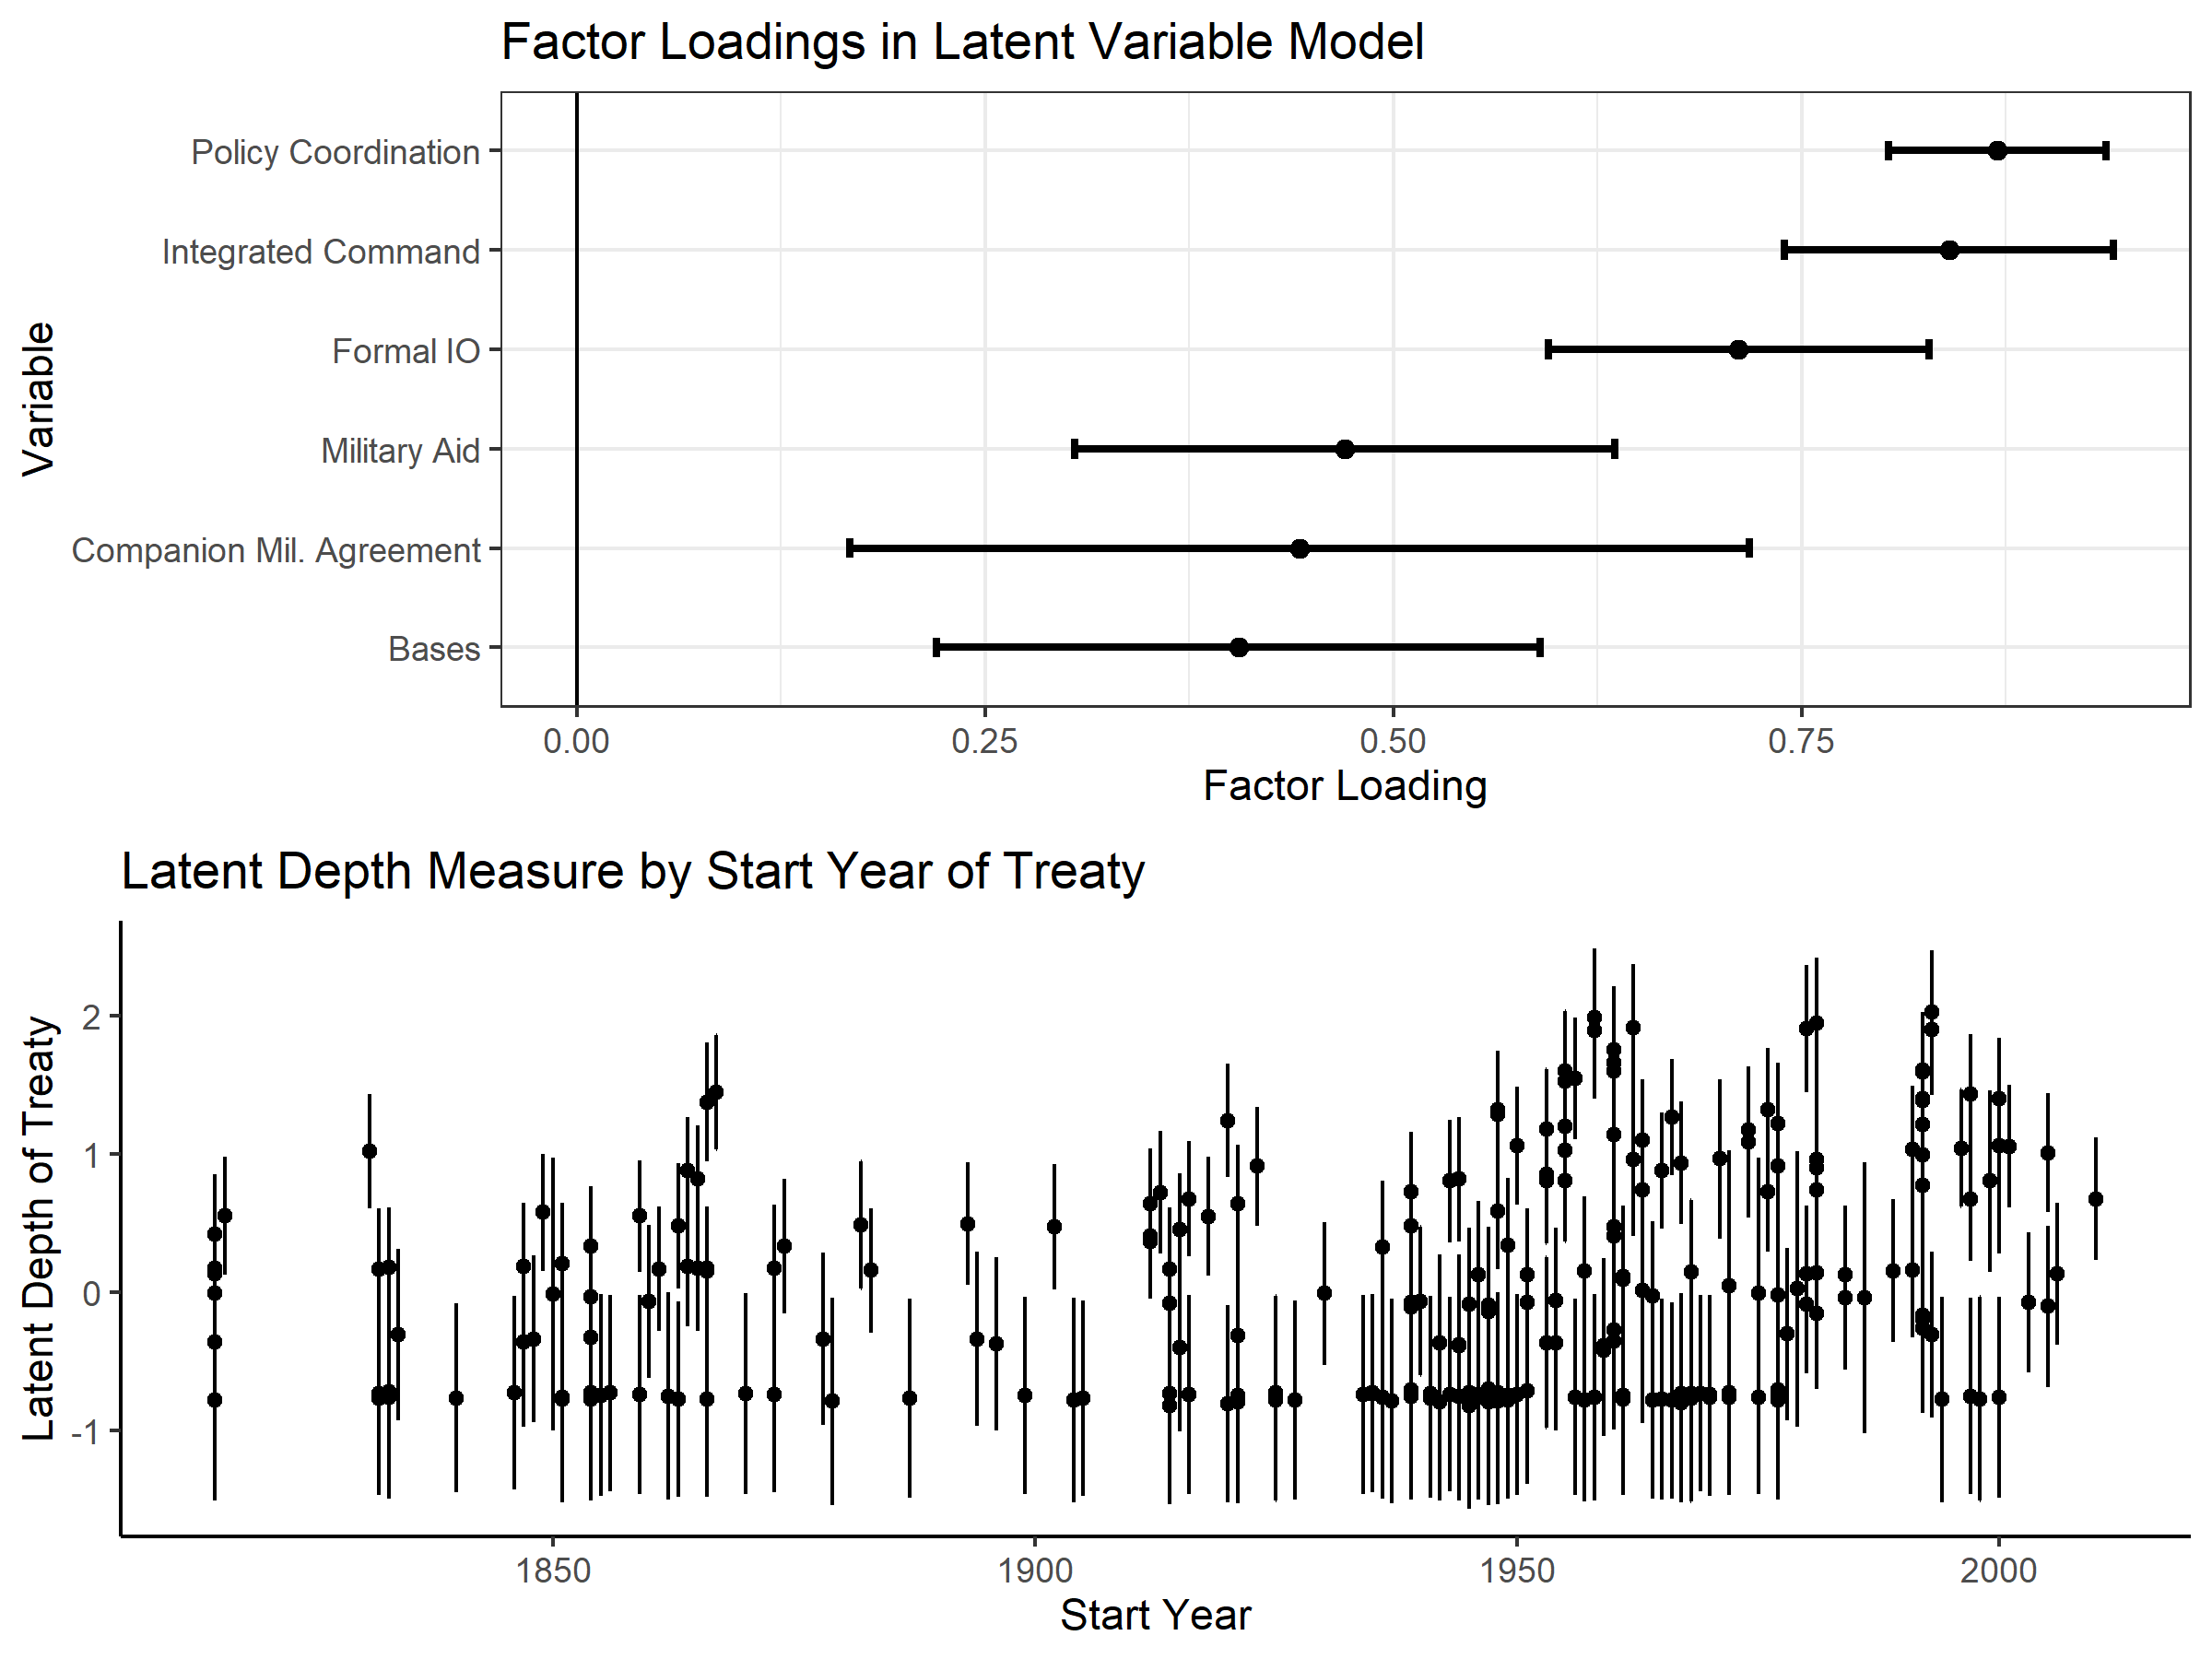
\includegraphics[width=0.95\textwidth]{../figures/loadings-measure.png}
\caption{Factor Loadings and posterior distributions of latent alliance treaty depth measure.}
\label{fig:loadings-measure}
\end{figure}


Based on these factor loadings, the measurement model predicts the likely value of treaty depth. 
The distribution of depth is summarized by the bottom panel of \autoref{fig:loadings-measure}. 
There is substantial variation in alliance treaty depth. 
Around half of all formal alliance treaties have an least some depth, and when states add depth, there is a wide range of treaty designs.
I measure treaty depth using the posterior mean of the latent depth posterior for each alliance. 
This summarizes the central tendency of latent treaty depth. 


The other outcome variable is a dummy indicator of unconditional military support. 
Using ATOP's information on whether defensive or offensive promises are conditional on specific locations, adversaries, or non-provocation, I set this variable equal to one if the treaty placed no conditions on military support.
123 of 289 alliances in the data offer unconditional military support. 


The key independent variable is the average democracy of alliance members at the time of treaty formation. 
I use the POLITY measure of political institutions to measure democracy, and calculate the average polity score of alliance members in the first year to predict alliance treaty design. 
This measure is a useful way to conceptualize the influence of domestic political regimes on alliance negotiations. 
As it increases, the average regime type of alliance members becomes more democratic. 


% Justify this approach
A common alternative measure of allied democracy is a dummy variable which is equal to one if both alliance members have a polity score greater than 5.\footnote{Only 25 of the 285 alliances in my data clear this joint democracy threshold.}
I prefer the average measure to this dummy for three reasons.
First, it translates better to multilateral alliances. 
Moreover, joint democracy is a slightly different concept, and I expect that domestic regimes affect alliances between democracies and non-democracies, even if such alliances are unusual \citep{Leeds1999}.
Finally, the average measure allows me to make inferences about highly democratic, highly autocratic, and mixed alliances. 



\subsection{Estimation Strategy}

I use several statistical models to examine how political regimes affect treaty depth. 
I start with separate models of treaty depth and unconditional military support. 
But because common unobserved factors may affect depth and conditionality, I specify a statistical model with two equations and correlated errors.
This approach is analogous to a bivariate probit model, but it is not fully recursive, because I do not use depth or unconditional military support as endogenous predictors of the other factor. 
One model predicts the probability of unconditional military support, and the other predicts treaty depth.


To model unconditional military support, I fit a binomial model with probit link function. 
The average democracy measure is the key independent variable, and I control for a range of other factors that are likely correlates of unconditional military support and allied democracy. 
Key controls include dummy indicators of asymmetric alliances between non-major and major powers and symmetric alliances between major powers \citep{Mattes2012}\footnote{This leaves symmetric alliances between major powers as the base category} as well as the average threat among alliance members at the time of treaty formation \citep{LeedsSavun2007}. 
I also control for foreign policy similarity \citep{Benson2012} using the minimum value of Cohen's $\kappa$ in the alliance \citep{Hage2011}.
Using the ATOP data \citep{Leedsetal2002}, I control for asymmetric treaty obligations, the number of alliance members, whether any alliance members were at war and the year of treaty formation. 
To capture the role of issue linkages in facilitating alliance agreements \citep{Poast2012, Poast2013}, I include a dummy indicator of whether the alliance addressed economic issues.  
Last, I include a count of foreign policy concessions in the treaty, because concessions can facilitate alliance negotiations \citep{Johnson2015}. 


The model of treaty depth controls for the same set of variables as the model of unconditional support. 
All these variables could conceivably alter the need for additional reliability from treaty depth. 
Modeling depth is more complicated because the latent measure is skewed.
To facilitate model fitting, I transformed latent depth to range between zero and one and modeled it with a beta distribution.\footnote{I also considered log-logistic, Dagum and inverse Gaussian distributions for the outcome, but AIC and residuals showed that the beta model fit best.}
The flexibility of the beta distribution helps predict mean latent depth.\footnote{The beta distribution also facilitates fitting models that account for uncertainty in the latent measure, which I will address in a later version of the paper.} 


First, I fit the models of unconditional support and treaty depth separately. 
I then fit them simultaneously using a generalized joint regression model (GJRM) \citep{Braumoelleretal2018}.
GJRM uses copulas to model correlations in the error terms of multiple equation models, which makes it more flexible than parametric models and facilitates causal inference. 
Adjusting for unobserved correlations between depth and unconditional military support ensures accurate inferences about democracy and other covariates. 
Copulas are distributions over functions, and relax potentially problematic assumptions about the shape of the correlation in the error terms. 
I fit models with all copulas, and selected the best-fitting model using AIC, conditional on that estimator having converged.\footnote{GJRM is estimated with maximum likelihood, and diagnostics for the gradient as well as the information matrix suggest that the models converged.} 
The Plackett copula provides the best model fit.


% justify this choice more
A third equation models heterogeneity in the error term correlations using the start year of the alliance. 
In particular, I suspect that correlations in unobservable factors between treaty depth and unconditional promises of military spending vary over time. 
Using the start year of the treaty to predict error correlations captures common unobserved shocks from the international context. 
For example, \citet{Kuo2019} shows how European politics led to a proliferation of secret alliances before World War I. 


GJRM also easily estimates non-linear relationships with smoothed terms. 
I estimated smoothed terms for democracy, mean threat and the start year of the alliance to capture potential non-linear relationships.\footnote{Fitting models with foreign policy similarity smoothed returned effective degrees of freedom = 1, which suggests a linear fit is equivalent. The smoothed terms for average democracy are also linear, but I retain the smoothed terms to facilitate substantive predictions.}  
Higher effective degrees of freedom on the smoothed terms indicate non-linear relationships, and chi-squared statistics give approximate statistical significance. 
In the next section, I summarize the results of the analysis. 



\section{Results}


My findings are partially consistent with the claim that increasing democracy in an alliance leads to treaties with conditional support and greater depth. 
I find consistent evidence that democracy increases treaty depth and weaker evidence that democracies offer conditional alliances. 
To begin, I offer some descriptive statistics.
Then, I present inferences from separate models. 
Last, I show evidence from the joint model. 


First, unconditional alliances tend to have lower democracy. 
The average of polity scores among alliances with unconditional military support is -1.4. 
Conversely, the average of the polity scores in alliances with conditional obligations is 1.62.\footnote{Based on a t-test, the difference between these values is statistically significant.} 
There is also a moderate positive correlation between average alliance democracy at the time of formation and treaty depth. 


% plot 
\autoref{fig:democ-combo} shows how the average democracy of alliance members at the time of alliance formation differs as the mix of unconditional military support and high treaty depth in treaty design changes.
In \autoref{fig:democ-combo}, each quadrant corresponds to part of \autoref{tab:str-table}.
To divide the latent depth measure, I classified deep alliances as treaties with a latent depth score above the median value. 
On average, conditional alliances with high depth have higher polity scores. 
Conversely, unconditional alliances with little depth have the lowest average polity scores. 


\begin{figure}[hbtp]
\centering
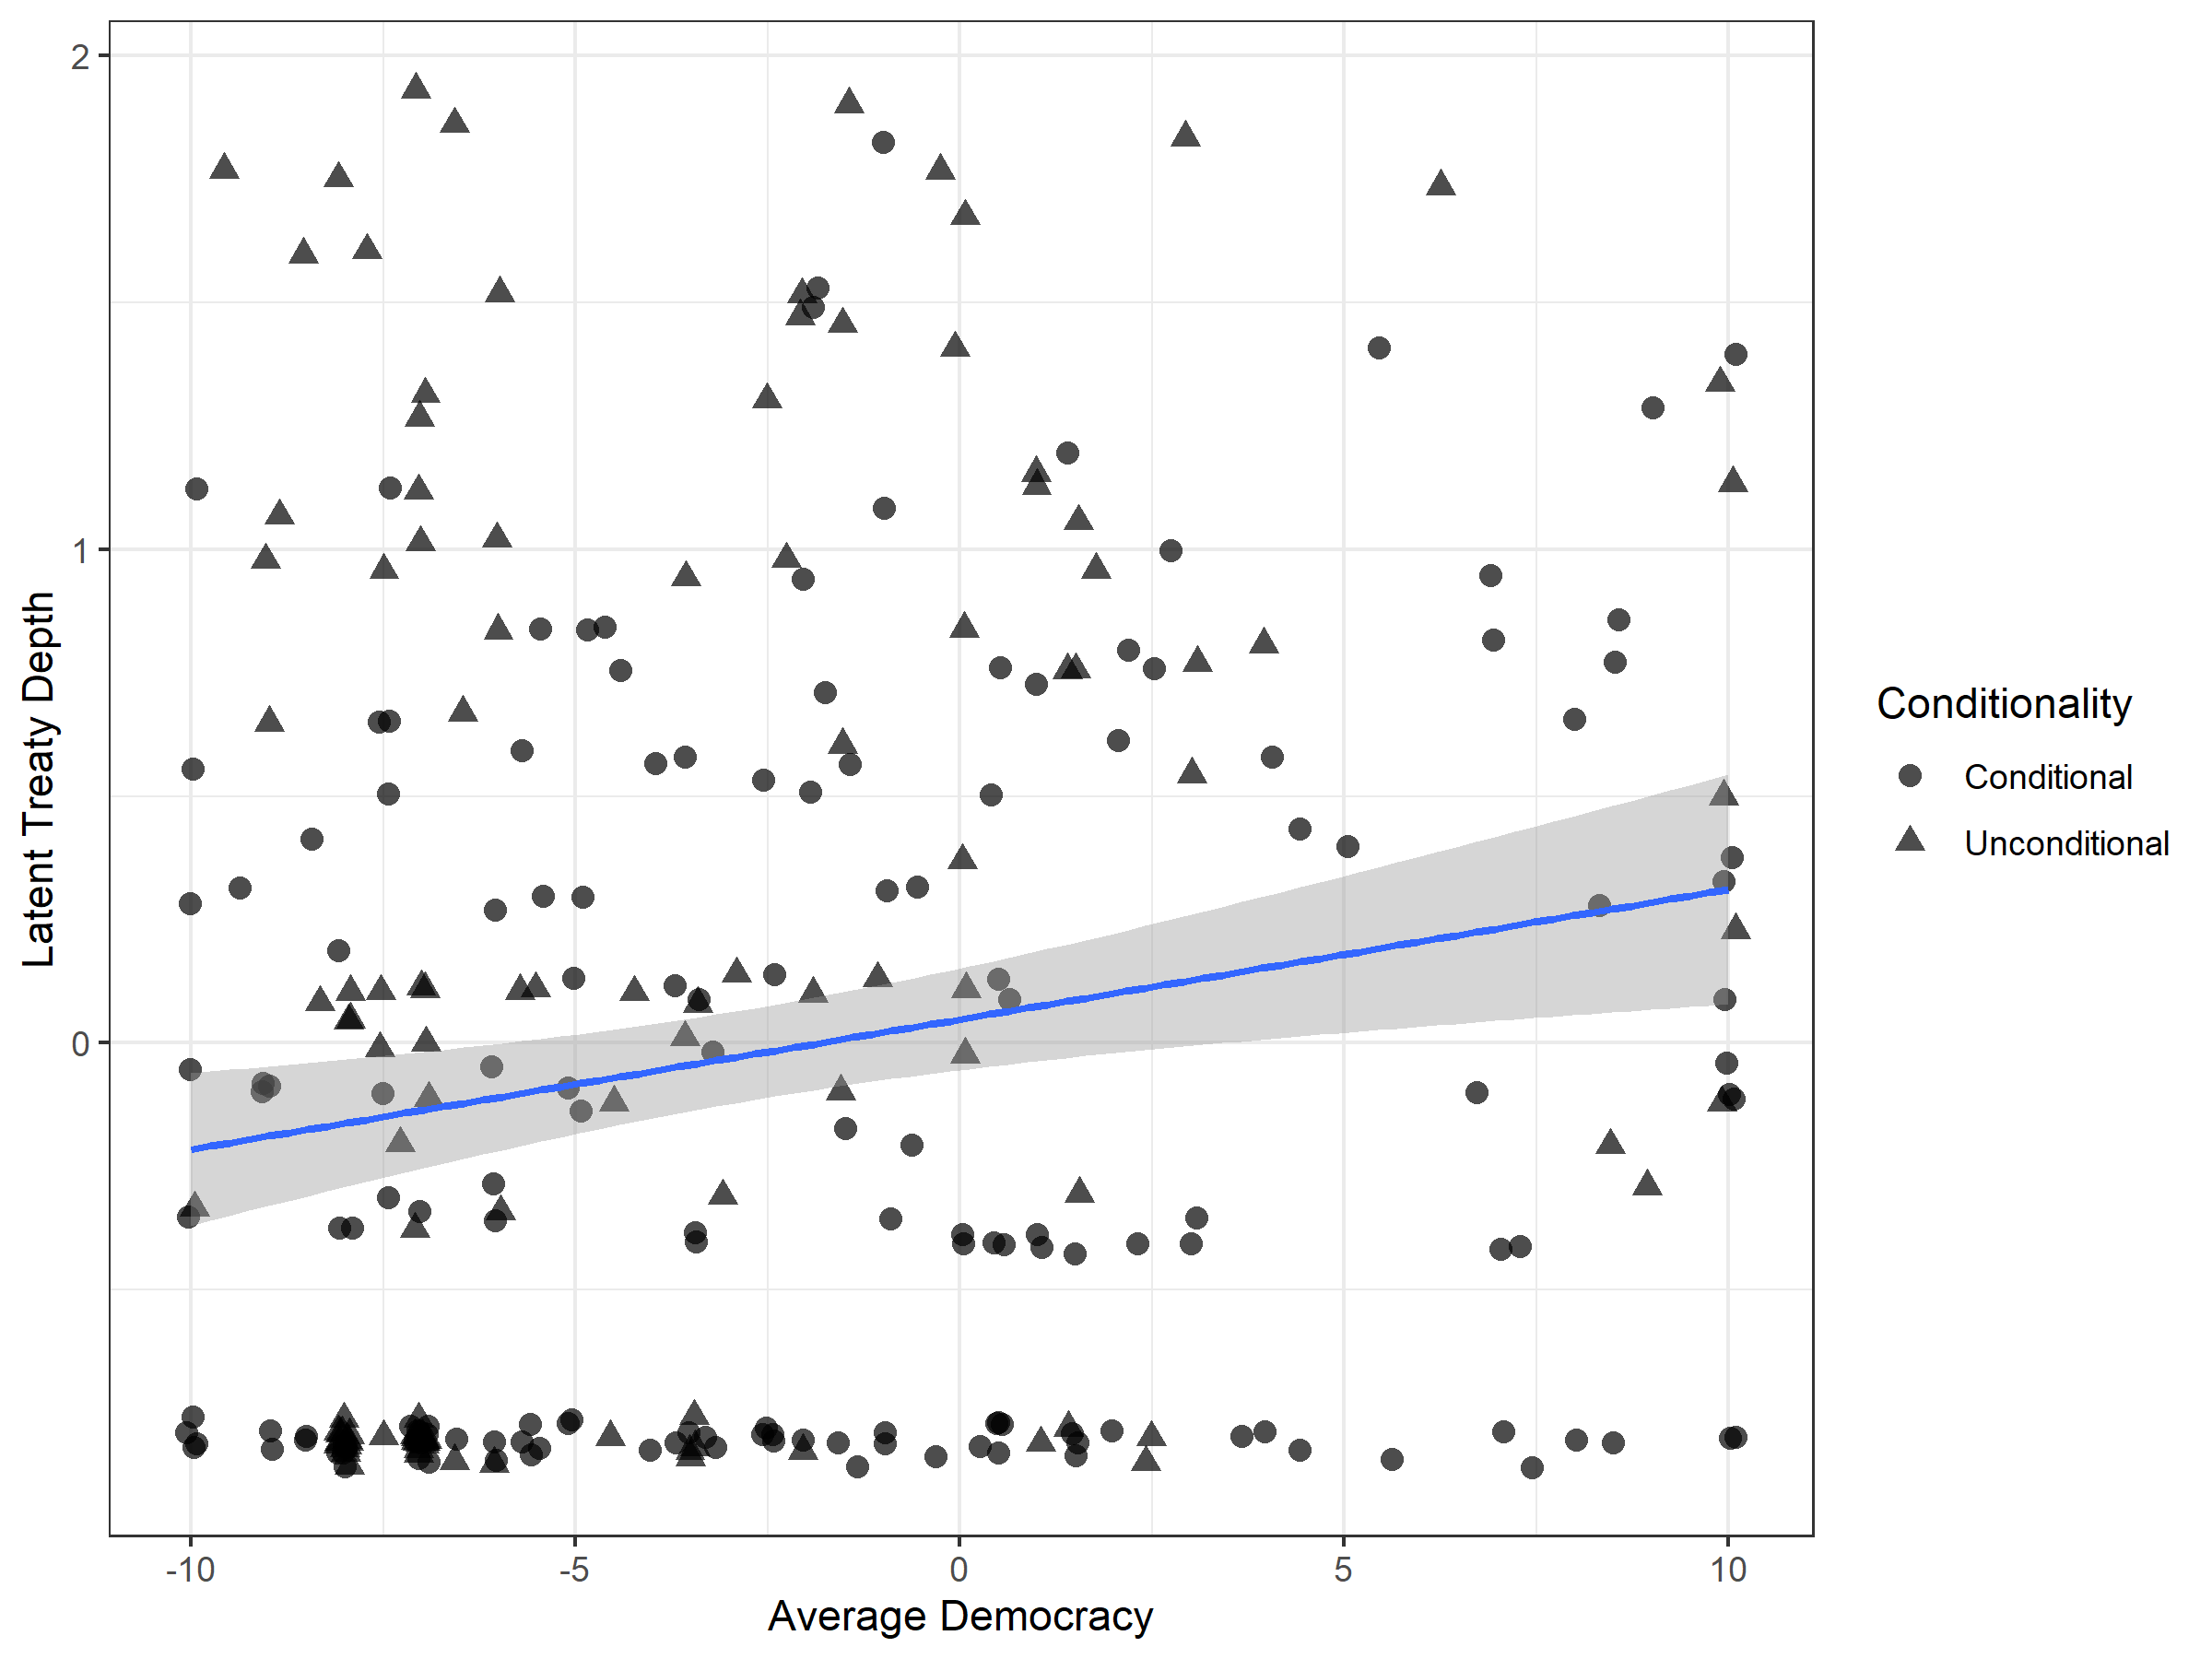
\includegraphics[width=0.95\textwidth]{../figures/democ-combo.png}
\caption{Average of the average polity score in four groups of alliance from 1816 to 2016. Divisions between alliances based on unconditional military support and treaty depth. Darker quadrants mark a higher average democracy score for that group of alliances, and the text in each box gives the precise value. }
\label{fig:democ-combo}
\end{figure}


These descriptive results do not adjust for potential confounding factors, however.
I now describe results from statistical models of depth and unconditional military support, starting with separate models. 
Results from independent models of depth and conditionality largely support the hypotheses. 
\autoref{tab:separate-models} shows results from a beta model of treaty depth and a binomial model of unconditional military support with a probit link function. 
The results are largely as expected, but the findings are somewhat weak.
For both outcomes, the 95\% confidence interval barely overlaps zero.  


\begin{table}[!htbp] \centering 
  \caption{Separate Models of Treaty Depth and Unconditional Military Support in Offensive and Defensive Alliances: 1816 to 2007.} 
  \label{tab:separate-models} 
\begin{tabular}{@{\extracolsep{5pt}}lcc} 
\\[-1.8ex]\hline 
\hline \\[-1.8ex] 
 & \multicolumn{2}{c}{\textit{Dependent variable:}} \\ 
\cline{2-3} 
\\[-1.8ex] & Latent Depth (rescaled) & Unconditional Military Support \\ 
\\[-1.8ex] & \textit{beta} & \textit{probit} \\ 
\\[-1.8ex] & (1) & (2)\\ 
\hline \\[-1.8ex] 
 Average Polity Score & 0.025$^{}$ & $-$0.035$^{}$ \\ 
  & ($-$0.001, 0.051) & ($-$0.072, 0.002) \\ 
  Foreign Policy Concessions & $-$0.066 & 0.004 \\ 
  & ($-$0.219, 0.087) & ($-$0.214, 0.222) \\ 
  Number of Members & 0.020 & $-$0.028 \\ 
  & ($-$0.006, 0.047) & ($-$0.074, 0.019) \\ 
  Wartime Alliance & $-$0.300$^{}$ & $-$0.950$^{}$ \\ 
  & ($-$0.649, 0.049) & ($-$1.568, $-$0.333) \\ 
  Asymmetric Obligations & 0.218 & 0.075 \\ 
  & ($-$0.123, 0.559) & ($-$0.427, 0.577) \\ 
  Asymmetric Capability & 0.374 & 0.607 \\ 
  & ($-$0.094, 0.842) & ($-$0.264, 1.479) \\ 
  Non-Major Only & 0.293 & 1.111$^{}$ \\ 
  & ($-$0.213, 0.798) & (0.224, 1.997) \\ 
  Average Threat & 1.175$^{}$ & 1.564$^{}$ \\ 
  & (0.310, 2.040) & (0.239, 2.888) \\ 
  Foreign Policy Disagreement & 0.166 & 0.368 \\ 
  & ($-$0.286, 0.617) & ($-$0.324, 1.060) \\ 
  Start Year & 0.004$^{}$ & 0.015$^{}$ \\ 
  & (0.0002, 0.007) & (0.010, 0.021) \\ 
  Constant & $-$8.565$^{}$ & $-$31.678$^{}$ \\ 
  & ($-$15.381, $-$1.749) & ($-$43.109, $-$20.248) \\ 
 \hline \\[-1.8ex] 
Observations & 277 & 277 \\ 
Log Likelihood & 53.807 & $-$131.527 \\ 
\hline 
\hline \\[-1.8ex] 
\textit{Note:}  & \multicolumn{2}{r}{95\% Confidence Intervals in Parentheses.} \\ 
\end{tabular} 
\end{table} 

Although the results from separate models are somewhat as expected, these models do not account for unobserved correlations between depth and conditions on military support. 
This omission could easily affect inferences. 
I now report the results of the joint analysis of depth and unconditional military support. 
\autoref{fig:results-democ-avg} plots the estimated effect of average democracy on the two outcomes. 


\begin{figure}[hbtp]
\centering
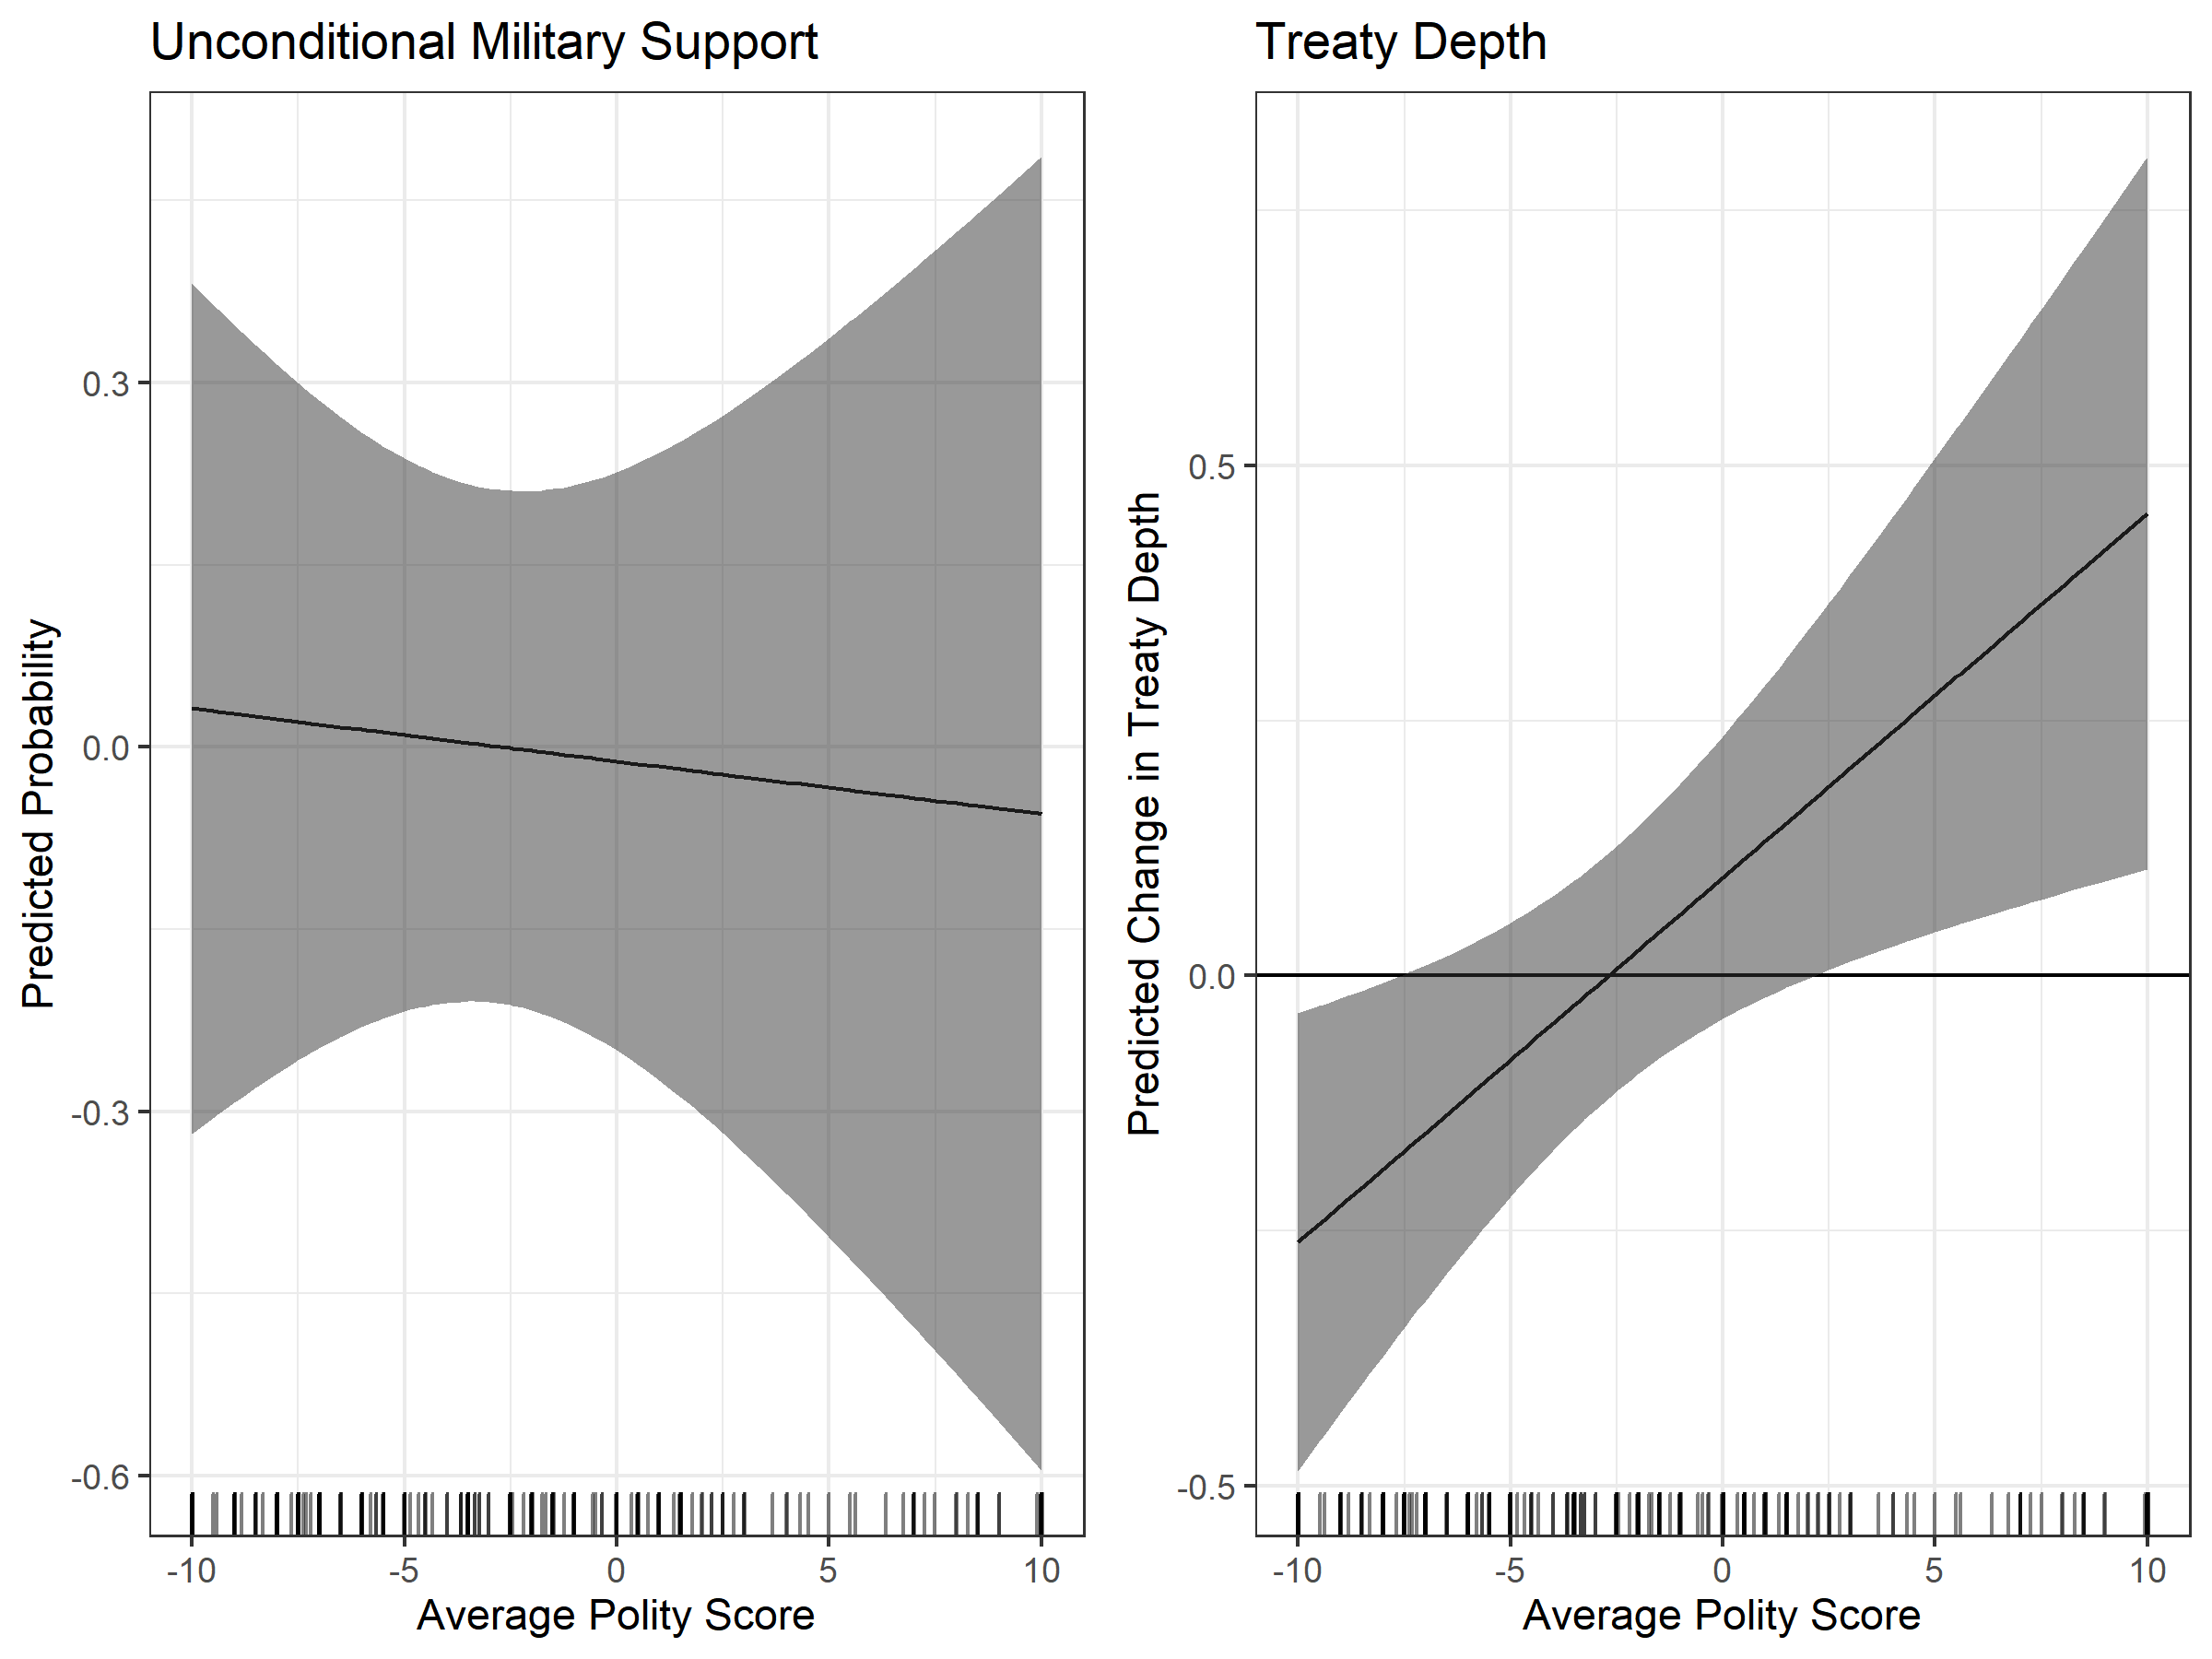
\includegraphics[width=0.95\textwidth]{../figures/results-democ-avg.png}
\caption{Predicted probabilities of unconditional military support and predicted changes in treaty depth across the range of average alliance democracy. The line marks predicted values, and the shaded areas encapsulate the standard errors. The rug plot on the x-axis marks observed values of allied democracy. Predictions based on the smoothed terms from the joint generalized regression model.}
\label{fig:results-democ-avg}
\end{figure}


The left-hand plot of \autoref{fig:results-democ-avg} shows the association between the average democracy of alliance members and the predicted probability of unconditional military support. 
This result is far weaker than I expected.  
There is no clear difference between alliances with a low average polity score and a high average polity score. 
These results contradict previous findings \citep{Mattes2012, Chibaetal2015}.


The right-hand plot in \autoref{fig:results-democ-avg} shows a positive relationship between democracy at the time of alliance formation and treaty depth.
Substantial democracy in an alliance is associated with greater treaty depth. 
Highly autocratic alliance membership decreases treaty depth, on the other hand. 
This trend of greater depth as the democracy of alliance members rises matches the treaty depth hypothesis. 


There are some other interesting inferences in the control variables, which I present in in \autoref{tab:gjrm-res}. 
This table contains results from both equations of the GJRM model, and marks smoothed terms with the letter s. 
I first describe the unconditional military support results before turning to the correlates of treaty depth. 
Asymmetric capability in an alliance and symmetric alliances between non-major powers are more likely to include unconditional military support than symmetric major power alliances. 
I also find that the number of members and wartime alliances reduce the probability of unconditional military support. 
Asymmetric capability and the number of alliance members both increase depth. 
Last, threat and the year of alliance formation increase unconditional military support and treaty depth in a nonlinear fashion. 

\begin{table}[ht]
\centering
\begin{tabular}{lrrrr}
  & \multicolumn{2}{c}{Uncond. Mil. Support} & \multicolumn{2}{c}{Latent Depth}\\ \hline
   & Estimate & Std. Error & Estimate & Std. Error \\ 
  \hline
  Economic Issue Linkage & 0.1388084 & 0.2001982 & 0.0308515 & 0.1486703 \\ 
  FP Concessions & -0.0908525 & 0.1269686 & -0.0577831 & 0.0835579 \\ 
  Number of Members & -0.0816235 & 0.0291638 & 0.0229947 & 0.0134521 \\ 
  Wartime Alliances & -0.6544537 & 0.3347940 & -0.0629485 & 0.1882251 \\ 
  Asymmetric Obligations & -0.2045893 & 0.2270098 & 0.1582906 & 0.1591976 \\ 
  Asymmetric Capability & 0.8424676 & 0.3600156 & 0.4099531 & 0.2133934 \\ 
  Non-Major Only & 1.5431343 & 0.3736788 & 0.1103324 & 0.2367420 \\ 
  FP Disagreement & 0.1344295 & 0.3530185 & 0.3349221 & 0.2258318 \\ 
  s(Avg. Polity Score) & 1.0000000 & $\chi^2$ = 0.0498925 & 1.0000000 & $\chi^2$ = 7.6255379 \\ 
  s(Mean Threat) & 7.0969555 & $\chi^2$ = 30.6821338 & 1.0000000 & $\chi^2$ = 19.3673775 \\ 
  s(Start Year) & 4.9194037 & $\chi^2$ = 43.1177456 & 7.7563199 & $\chi^2$ = 50.1378368 \\ 
  (Intercept) & -0.9848832 & 0.4619137 & -1.1754086 & 0.2479738 \\ 
   \hline
\end{tabular}
\caption{Results from joint generalized regression model of treaty depth and unconditional military support. 
          Smoothed terms for democracy, mean threat and the start year of the treaty report the effective degrees of freedom and the chi-squared term. 
                     The unconditional military support model is a binomial GLM with a probit link function. 
                     The treaty depth model is a beta regression. 
                     The error correlation between the two processes is modeled with a Plackett copula.} 
\label{tab:gjrm-res}
\end{table}


The difference between the results in \autoref{fig:results-democ-avg} and \autoref{tab:gjrm-res} and the single-equation models in \autoref{tab:separate-models} is the result of adjusting for correlations in the error terms of the two equations. 
Kendall's $\tau$ measures the strength of the correlation between the errors, and is a function of the $\theta$ parameter.
I used the start year of the alliance to predict differences in $\theta$, which affects correlations in unobservables between depth and unconditional military support. 
\autoref{fig:results-error} plots the smoothed term I used to predict the correlation in the error terms between treaty depth and unconditional military support. 
The predicted values in the top panel of \autoref{fig:results-error} are on the scale of $\theta$. 
In the bottom panel, I plot predicted $\tau$ values against the start year of the alliance. 


\begin{figure}[hbtp]
\centering
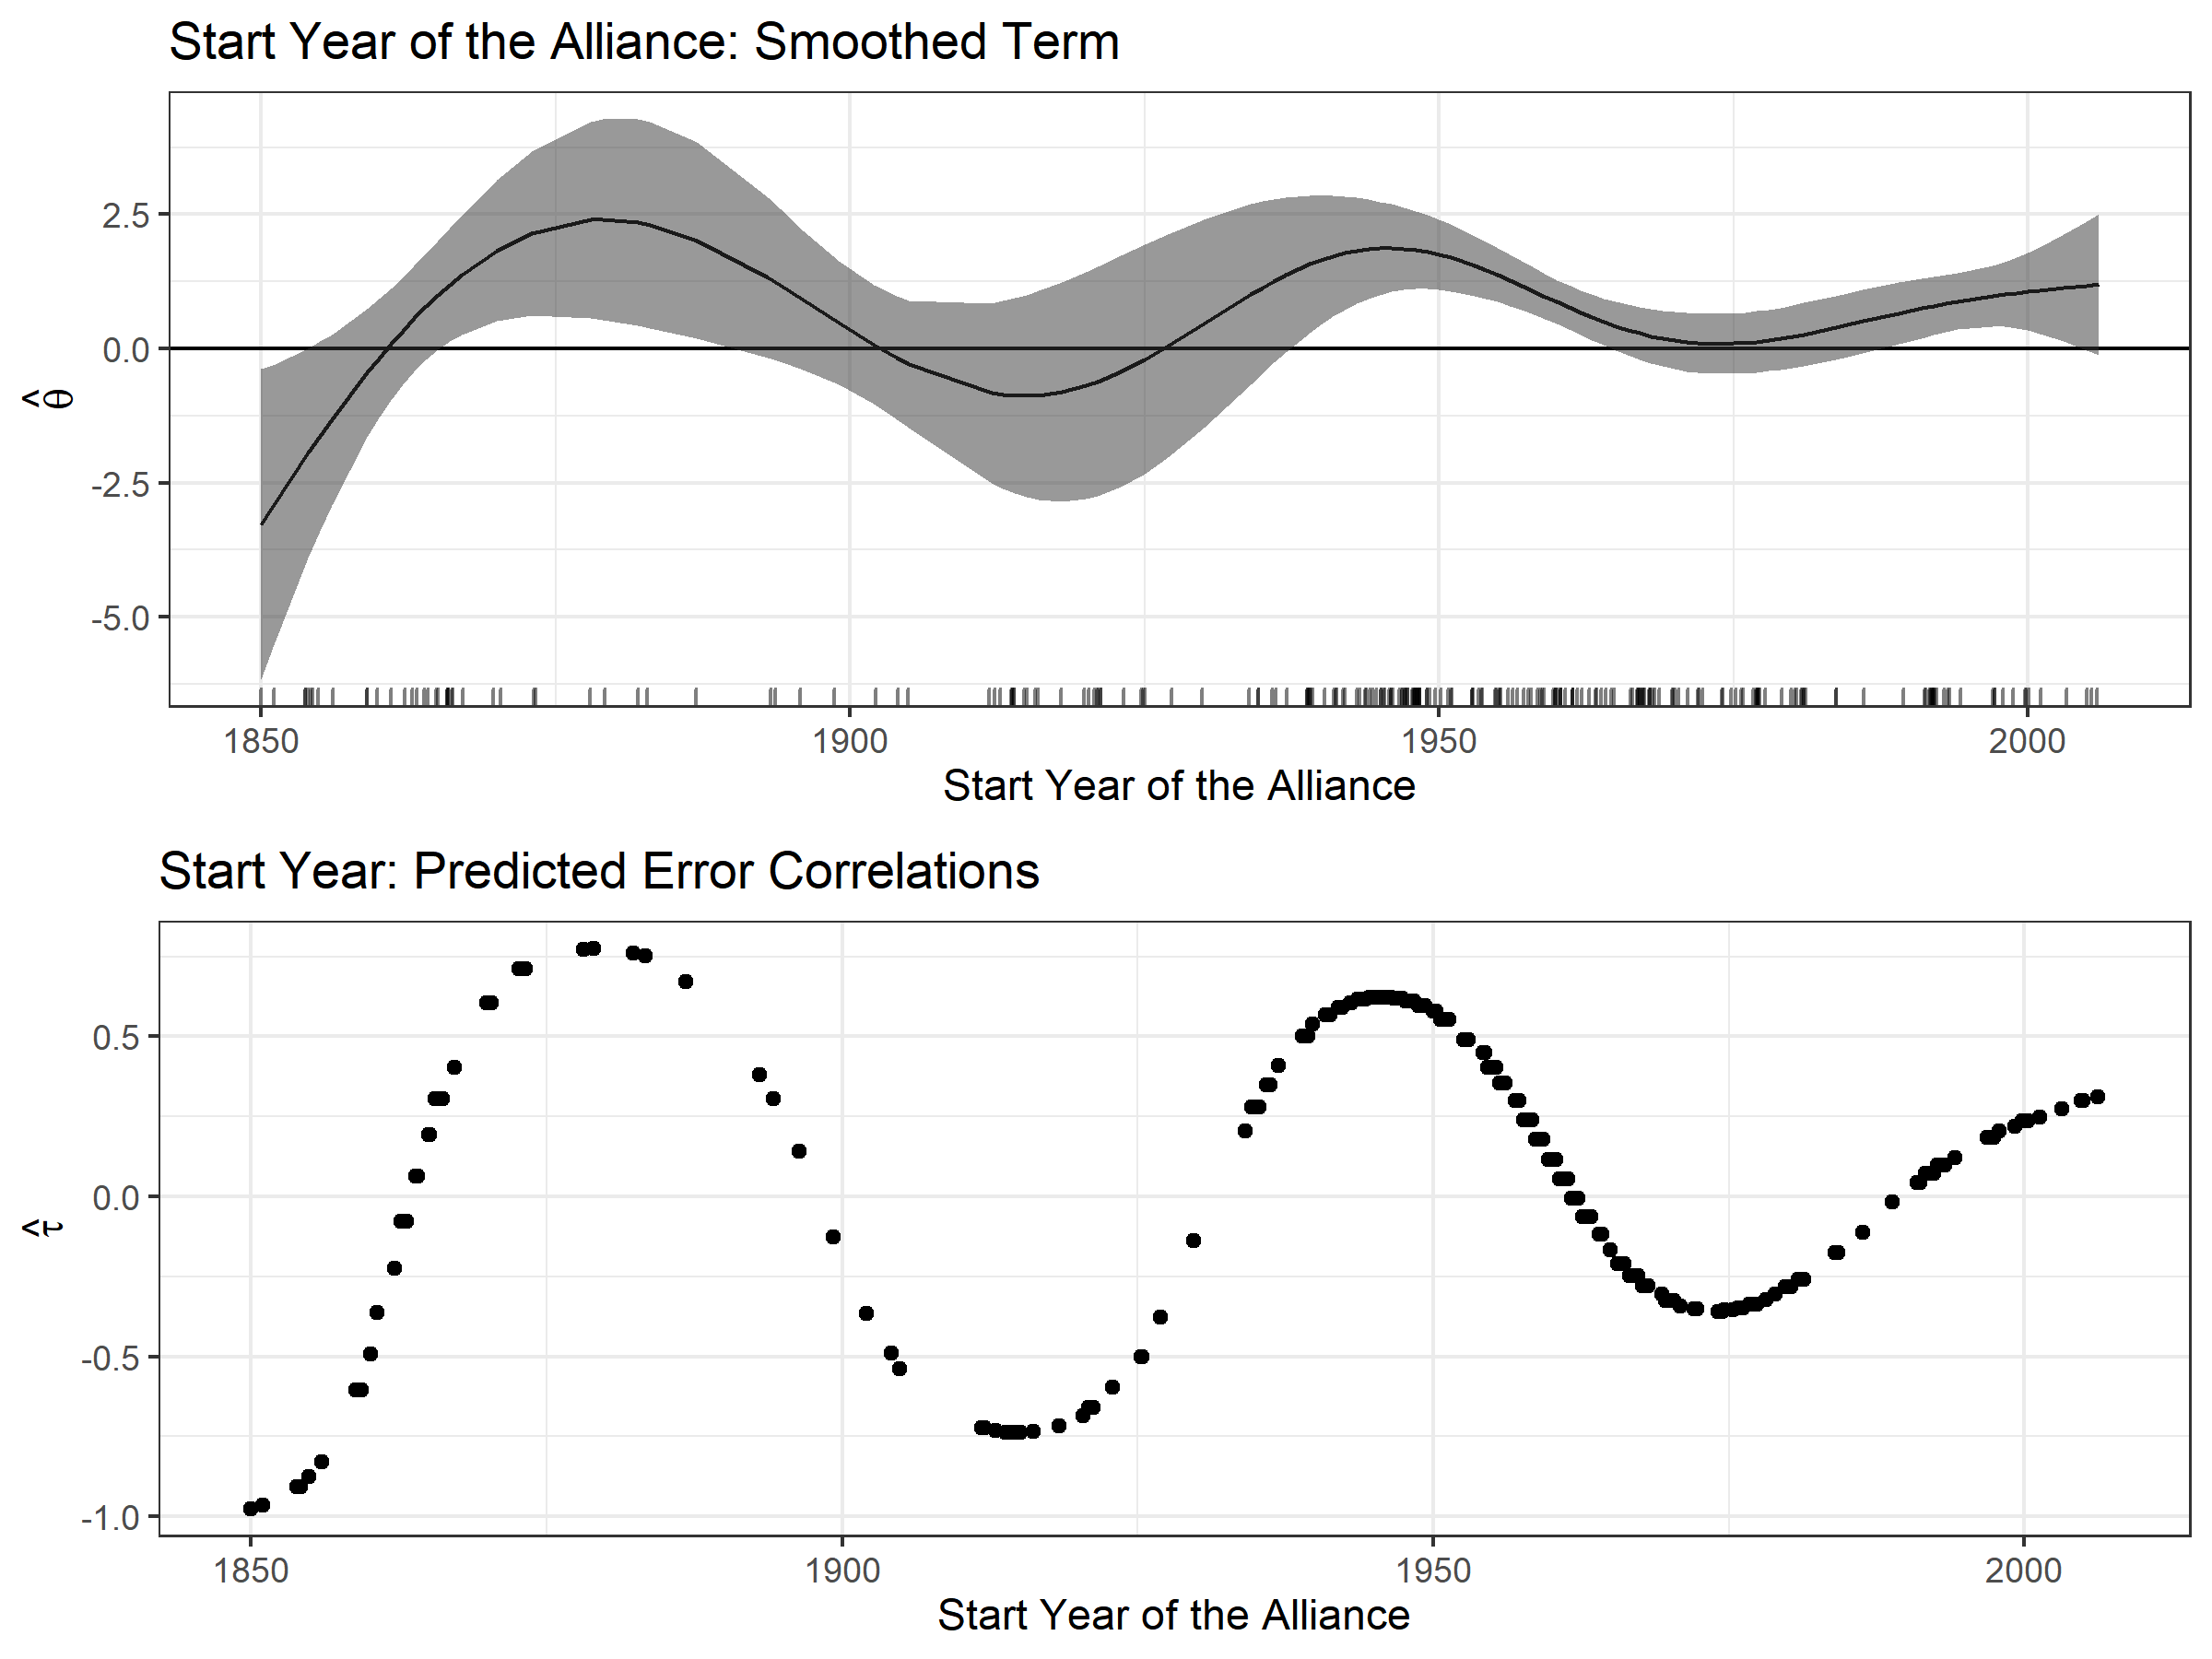
\includegraphics[width=0.95\textwidth]{../figures/results-error.png}
\caption{Predicted association between the errors of the unconditional military support and treaty depth models by the start year of the alliance. There is limited alliance data before 1850, which dramatically increases uncertainty in the smoothed term. To make the plot more legible I present predictions from after 1850. The rug plot on the x-axis in the top row marks the distribution of alliances. Each point in the bottom row is an estimated $\tau$, one for each of the 277 observations.}
\label{fig:results-error}
\end{figure}


As \autoref{fig:results-error} shows, the predicted association between the errors varies heavily by year. 
The association is positive for part of the period between 1850 and 1900, before turning more negative between 1900 and 1950. 
During World War II depth and unconditional military support are positively associated. 
In general, the magnitude and direction of estimated correlation between depth and unconditional military support in unobserved factors $\tau$ changes dramatically over time.  


Again, correlations between unobserved factors are responsible for differences in results between the joint model and the separate models. 
After accounting for correlations in the error terms of the unconditional military support and treaty depth models, I find little connection between political regimes and the probability of unconditional military support. 
Existing findings are sensitive to confounding from unobserved factors, which may be connected to shifts in the international context over time. 
 

The aggregate patterns in these statistical results give mixed evidence for the argument. 
They do not track the process of alliance treaty negotiation, however. 
To corroborate my theoretical claim that democracies prefer depth to unconditional support, I now offer a brief case study of the alliance negotiations behind NATO. 


\subsection{Case Study: NATO}


I focus on NATO in this case study for two reasons. 
First, it provides a helpful illustration of the process behind the aggregate patterns in the statistical analysis. 
US foreign policy after World War II exemplifies the tendency of democratic states to use treaty depth for reassurance, while also providing conditional obligations.  
Most US alliances have conditional promises of military support and some depth, and NATO fits this pattern.
Second, NATO is also perhaps the most important alliance in international politics, so understanding how it was designed is worthwhile. 


After the end of World War II, the US sought a way to protect Europe from the USSR. 
There were two challenges in negotiating the alliance, however.
First, as \citet{Poast2019a} details, NATO members disagreed over how to define the North Atlantic area, which was a key condition on military support. 
The US and other states argued about whether France's Algerian colony and Italy fell under the promises of support in the alliance. 
Second, the promises of military support in Article V of NATO depend on domestic political processes.\footnote{\citet{Benson2012} calls this kind of commitment a ``probablistic'' obligation.} 
Isolationists in the US Senate feared that an alliance would force America to intervene automatically if partners were attacked, bypassing the power of Congress to declare war \citep[pg. 280-1]{Acheson1969}.
Therefore Article V states that if one member is attacked the others ``will assist the Party or Parties so attacked by taking forthwith, individually and in concert with the other Parties, \emph{such action as it deems necessary} (emphasis mine).'' 
Military support was and is not guaranteed by the NATO treaty. 
Secretary of State Dean Acheson stated as much in a March 1949 press release, where he said that Article V ``does not mean that the United States would automatically be at war if one of the nations covered by the Pact is subject to armed attack'' \citep{Acheson1949}. 


The absence of automatic US involvement increased demand for reassurance by European allies. 
Europeans feared that if the Soviets invaded, the US would decide not to fight. 
Therefore, the US took other measures to reassure NATO allies. 
A 1951 presentation by Dean Acheson to Dwight Eisenhower argued European allies ``fear the inconstancy of United States purpose in Europe. ... These European fears and apprehensions can only be overcome if we move forward with determination and if we make the necessary full and active contribution in terms of both military forces and economic aid'' \citep[pg. 3]{Acheson1951}. 


The first part of reassurance was the creation of the Atlantic Council, which is an international organization and the only source of depth in the NATO treaty itself. 
The United States used participation in this organization and other efforts to coordinate collective defense and increase the perceived reliability of the alliance. 
By investing in the Atlantic Council and related joint military planning, the US addressed European fears of abandonment. 
For example, US officials thought that the British Foreign Minister viewed US provision of a supreme commander in Europe as ``a stimulus to European action'' \citep{Acheson1950}. 


Many Senators also opposed military aid to Europe \citep[pg 285]{Acheson1969}, which limited efforts to add further treaty depth. 
Bilateral agreements on troop deployments then became another instrument of reassurance. 
In 1950 the Germans formally requested clarification on whether an attack on US forces in Germany would be treated as an armed attack on the US- which the US said it would \citep[pg. 395]{Acheson1969}.  
Even after agreeing to deploy troops, US policymakers hoped Europeans would soon provide more for their own defense, while acknowledging the US ``should not dictate what they shall do'' \citep[pg. 2]{Johnson1950}. 
These bilateral arrangements and basing rights are not covered in the NATO treaty, but they added substantial depth.\footnote{This reveals an important limitation of my statistical approach.}  


% Sum up 
NATO negotiations reveal the tendency of democracies to add conditions on military support, but then use treaty depth to reassure their allies. 
The United States preferred conditional military support, but was willing to invest in deep military cooperation. 
The Atlantic Council and bureaucratic machinery of the NATO treaty are the basis for substantial defense cooperation. 
Therefore, though Article V is more limited than many realize, NATO is still a deep alliance. 
US alliances are not limited commitments, even if they rarely offer unconditional military support. 


\section{Discussion and Conclusion}


% main evidence for an indirect effect
The findings from the statistical models and case study of NATO provide inconsistent evidence. 
I find regular evidence that democracies tend to form deep alliances.
There is mixed evidence that allied democracy decreases the probability of unconditional military support, however. 
This challenges the conventional wisdom that democracies make limited alliance commitments.
The effect of democracy on conditions for military support may be weaker than previously thought and democracies often increase the depth of their alliances. 
Therefore, democracies often make moderate strength alliance commitments. 
Depth may even be a more salient source of security cooperation than unconditional military support. 


% Conclusion depends on how alliances and military spending are connected
I base most of my conclusions about democracy and unconditional military support on the joint model of depth and unconditional military support.
Without a joint model, I find the expected negative correlation between maximum democracy and unconditional military support.  
Inferences about democracy and other covariates depend on this theoretical and empirical choice to model depth and unconditional military support together. 
Again, I do note use treaty depth and unconditional military support to predict the other outcome. 
A fully recursive model that includes depth and unconditional military support as predictors requires valid instruments for identification.
Given the potential for biased findings from a weak instrument or one that violates the exclusion restriction, and lack of clear instruments for treaty depth, I am hesitant to employ a fully recursive model.  


% Therefore, sources of alliance credibility are rather entangled
My findings show how different aspects of alliance treaty design are related. 
\citet{BensonClinton2016} use measurement models to show this in a descriptive fashion, but my findings give a sense of the process behind different combinations of depth and conditions on military support. 
Previous research on the causes of alliance treaty design \citep{Benson2012, Mattes2012, Chibaetal2015} assumed different sources of alliance treaty reliability were independent. 
This approach can be informative, but it is incomplete- I find that treaty depth and unconditional military support are linked by changes in the international context. 


Although my argument and evidence offer some innovations, they have limitations. 
First, I only examine variation in formal treaty design. 
This omits the implementation of alliance promises, which may be deeper or shallower than the treaty language alone implies. 
As the NATO case study shows, formal treaty depth reflects practical depth, but it may miss some differences between alliances. 
At the same time, this study focuses on institutional design. 
Changes in realized alliance depth are a useful subject for future inquiry, but will require new data collection. 


The claims in this paper have consequences for several branches of scholarship. 
First, they speak to debates about whether democracies make more credible commitments. 
The effect of democracy on credibility can be divided into conditions on military support, treaty depth, and the direct effect of institutions and domestic politics. 
These may have competing or conditional effects, which could explain mixed findings about the credibility of democratic commitments \citep{Schultz1999, Leeds1999, Thyne2012, DownesSechser2012}.
The net effect of democracy on credible commitment in international relations requires further explanation. 


In general, studies of the consequences of alliance participation should account for alliance design and membership. 
This study shows that alliance membership and design are closely related. 
Estimating the impact of member characteristics alone, or treaty design alone, risks omitted variable bias. 


The key implication for scholarship is that alliance treaty design contains multiple related decisions. 
States do not provide depth or unconditional military support in isolation. 
Rather than address each part of treaty design piecemeal, scholars should examine relationships between the core aspects of treaty design. 
For example, future work might examine the connections between conditions on military support, treaty depth, and issue linkages.  
Any discussion of alliance treaty design must also situate these decisions in the process of treaty negotiations and what states are willing to offer.
As such, my findings support calls to correct the comparative neglect of negotiations in existing scholarship \citep{Poast2019a}. 


Last, alliances are an international institution, so some of the lessons from this work may apply to other institutions. 
There is an extensive literature on the design on international institutions \citep{DownesRocke1995, MartinSimmons1998, Koremenosetal2001, Koremenos2005, Thompson2010}.
My results suggest that scholars in this literature should consider how states use different means to achieve a goal for their formal institutions. 


In conclusion, democratic alliance membership increases treaty depth. 
Contrary to existing research, I find less evidence that democracies are more likely to offer unconditional alliances. 
Democracies do not make limited alliances, rather they establish credibility through costly signals with less exposure to domestic audience costs. 



\singlespace
 
\bibliography{../../../MasterBibliography} 





\end{document}